\chapter{Leader Election Algorithm}
\paragraph{}In this section, we present our leader election algorithm. The pseudocode for the algorithm is presented in Figures 1, 2 and 3. First, we provide an informal description of the algorithm, then, we present the details of the algorithm and the pseudocode, and finally, we provide an example execution. In the rest of this section, variable var of node u will be indicated as varu . For brevity, in the pseudocode for node u, variable varu is denoted by just var.
\section{Informal Description}
\paragraph{}Each node in the system has a 7-tuple of integers called a height. The directions of the edges in the graph are determined by comparing the heights of neighboring nodes: an edge is directed from a node with a larger height to a node with a smaller height. Due to topology changes nodes may lose some of their incident links, or get new ones throughout the execution. Whenever a node loses its last outgoing link because of a topology change, it has no path to the current leader, so it reverses all of its incident edges. Reversing all incident edges acts as the start of a search mechanism (called a reference level) for the current leader. Each node that receives the newly started reference level reverses the edges to some of its neighbors and in effect propagates the search throughout the connected component. Once a node becomes a sink and all of its neighbors are already participating in the same search, it means that the search has hit a dead end and the current leader is not present in this part of the connected component. Such dead-end information is then propagated back towards the originator of the search. When a node which started a search receives such dead- end messages from all of its neighbors, it concludes that the current leader is not present in the connected component, and so the originator of the search elects itself as the new leader. Finally, this new leader information propagates throughout the network via an extra “wave” of propagation of messages.
\paragraph{}In our algorithm, two of the components of a node’s height are timestamps record- ing the time when a new “search” for the leader is started, and the time when a leader is elected. In the algorithm in [15], these timestamps are obtained from a global clock accessible to all nodes in the system. In this paper, we use the notion of causal clocks (defined in Section 2.3) instead.
\paragraph{}One difficulty that arises in solving leader election in dynamic networks is dealing with the partitioning and merging of connected components. For example, when a connected component is partitioned from the current leader due to links going down, the above algorithm ensures that a new leader is elected using the mechanism of waves searching for the leader and convergecasting back to the originator. On the other hand, it is also possible that two connected components merge together resulting in two leaders in the new connected component. When the different heights of the two leaders are being propagated in the new connected component, eventually, some node needs to compare both and decide which one to adopt and continue propagating. Recall that when a new leader is elected, a component of the height of the leader records the time of the election which can be used to determine the more recent of two elections. Therefore, when a node receives a height with a different leader information from its own, it adopts the one corresponding to the more recent election.
\paragraph{}Similarly, if two reference levels are being propagated in the same connected component, whenever a node receives a height with a reference level different from its current one, it adopts the reference level with the more recent timestamp and con- tinues propagating it. Therefore, even though conflicting information may be prop- agating in the same connected component, eventually the algorithm ensures that as long as topology changes stop, each connected component has a unique leader.
\section{Nodes, Neighbors and Heights}
\paragraph{}First, we describe the mechanism through which nodes get to know their neighbors. Each node in the algorithm keeps a directed approximation of its neighborhood in Gchan as follows. When u gets a ChannelUp event for the channel from u to v, it puts v in a local set variable called formingu . When u subsequently receives a message from v, it moves v from its formingu set to a local set variable called Nu (N for neighbor). If u gets a message from a node which is neither in its forming set, nor in Nu , it ignores that message. And when u gets a ChannelDown event for the channel from u to v, it removes v from formingu or Nu , as appropriate. For the purposes of the algorithm, u considers as its neighbors only those nodes in Nu . It is possible for two nodes u and v to have inconsistent views concerning whether u and v are neighbors of each other. We will refer to the ordered pair (u, v), where v is in Nu , as a link of node u.
\paragraph{}Nodes assign virtual directions to their links using variables called heights. Each node maintains a height for itself, which can change over time, and sends its height over all outgoing channels at various points in the execution. Each node keeps track of the heights it has received in messages. For each link (u, v) of node u, u considers the link as incoming (directed from v to u) if the height that u has recorded for v is larger than u’s own height; otherwise u considers the link as outgoing (directed from u to v). Heights are compared using lexicographic ordering; the definition of height ensures that two nodes never have the same height. Note that, even if v is viewed as a neighbor of u and vice versa, u and v might assign opposite directions to their corresponding links, due to asynchrony in message delays.
\paragraph{}Next, we examine the structure of a node’s height in more detail. The height for each node is a 7-tuple of integers $((\tau , oid, r), \delta , (nlts, lid), id)$, where the first three components are referred to as the reference level ($RL$) and the fifth and sixth components are referred to as the leader pair ($LP$). In more detail, the components are defined as follows:
\begin{list}{--}{spacing}
	\item $\tau$ , a non-negative timestamp which is either $0$ or the value of the causal clock time when the current search for an alternate path to the leader was initiated.
	\item $oid$, is a non-negative value that is either $0$ or the $id$ of the node that started the current search (we assume node $ids$ are positive integers).
	\item $r$, a bit that is set to $0$ when the current search is initiated and set to $1$ when the current search hits a dead end.
	\item  $\delta$ , an integer that is set to ensure that links are directed appropriately to neighbors with the same first three components. During the execution of the algorithm $\delta$ serves multiple purposes. When the algorithm is in the stage of searching for the leader (having either reflected or unreflected $RL$), the $\delta$ value ensures that as a node u adopts the new reference level from a node $v$, the direction of the edge between them is from $v$ to $u$; in other words it coincides with the direction of the search propagation. Therefore, $u$ adopts the $RL$ of $v$ and sets its $\delta$ to one less than $v$’s. When a leader is already elected, the $\delta$ value helps orient the edges of each node towards the leader. Therefore, when node $u$ receives information about a new leader from node $v$, it adopts the entire height of $v$ and sets the $\delta$ value to one more than $v$’s. $-- nlts$, a non-positive timestamp whose absolute value is the causal clock time when the current leader was elected. $– lid$, the $id$ of the current leader. $-- id$, the node’s unique ID.
\end{list}
Each node $u$ keeps track of the heights of its neighbors in an array $height_u$, where the height of a neighbor node $v$ is stored in $height_u[v]$. The components of $height_u[v]$ are referred to as $(\tau ^v , oid^v , r^v , \delta ^v , nlts^v , lid^v , v)$ in the pseudocode.
\section{Initial States}
\paragraph{}The definition of an initial configuration for the entire system from Section 2.3 in- cluded the condition that each node be in an initial state according to its algorithm. The collection of initial states for the nodes must be consistent with the collection of initial states for the channels. Let $G_{init}$ chan be the undirected graph corresponding to the initial states of the channels, as defined in Section 2.3. Then in an initial configuration, the state of each node u must satisfy the following:
\begin{list}{--}{spacing}
	\item formingu is empty, – Nu equals the set of neighbors of u in Ginit chan
	\item heightu[u] = $(0, 0, 0, \delta _u , 0, l, u)$ where $l$ is the id of a fixed node in $u's$ connected chan (the current leader), and $\delta _u$ equals the distance from $u$ to $l$ in component in Ginit Ginit chan ,
	\item for each v in Nu , heightu[v] = heightv [v] (i.e., u has accurate information about v’s height), and
	\item Tu is initialized properly with respect to the definition of causal clocks.
\end{list}
\paragraph{}The constraints on the initial configuration just given imply that initially, each connected component of the communication topology graph has a leader; further- more, by following the virtual directions on the links, nodes can easily forward in- formation to the leader (as in TORA). One way of viewing our algorithm is that it maintains leaders in the network in the presence of arbitrary topology changes. In order to establish this property, the same algorithm can be executed, with each node initially being in a singleton connected component of the topology graph prior to any ChannelUp or ChannelDown events.
\section{Goal of the Algorithm}
\paragraph{}The goal of the algorithm is to ensure that, once topology changes cease, eventually each connected component of $G_{chan} ^{final}$ is “leader-oriented”, which we now define. Let CC be any connected component of $G_{chan} ^{final}$ . First, we define a directed version of $CC$, denoted $CC^{\longleftrightarrow}$, in which each undirected edge of $CC$ is directed from the endpoint with larger height to the endpoint with smaller height. We say that CC is leader-oriented if the following conditions hold:
\begin{enumerate}
	\item No messages are in transit in CC.
	\item For each (undirected) edge {u, v} in CC, if (u, v) is a link of u, then u has the correct view of v’s height.
	\item  Each node in CC has the same leader id, say $l$, where $l$ is also in $CC^{\longrightarrow}$. 
	\item  CC is a directed acyclic graph (DAG) with $l$ as the unique sink.
\end{enumerate}
A consequence of each connected component being leader-oriented is that the leader election problem is solved.
\section{Description of the Algorithm}
\paragraph{}The algorithm consists of three different actions, one for each of the possible events that can occur in the system: a channel going up, a channel going down, and the receipt of a message from another node. Next, we describe each of these actions in detail.
\paragraph{}First, we formally define the conditions under which a node is considered to be a sink:
\begin{list}{--}{spacing}
	\item SINK = $((\forall v \in N_u, LP_u ^v = LP_u ^u )$ and $(\forall v \in N_u, height_u[u] < height_u[v])$ and $(lid_u ^u = u))$. Recall that the $LP$ component of node $u’s$ view of $v’s$ height, as stored in $u's$ height array, is denoted $LP_u ^v$ , and similarly for all the other height components. This predicate is true when, according to $u's$ local state, all of $u's$ neighbors have the same leader pair as $u$, $u$ has no outgoing links, and $u$ is not its own leader. If node $u$ has links to any neighbors with different $LPs$, $u$ is not considered a sink, regardless of the directions of those links.
\end{list}
\paragraph{}$ChannelDown$ event: When a node u receives a notification that one of its incident channels has gone down, it needs to check whether it still has a path to the current leader. If the $ChannelDown$ event has caused $u$ to lose its last neighbor, as indicated by u’s N variable, then $u$ elects itself by calling the subroutine $ELECTSELF$. In this subroutine, node u sets its first four components to 0, and the LP component to $(nlts,u)$ where $nlts$ is the negative value of u’s current causal clock time. Then, in case u has any incident channels that are in the process of forming, u sends its new height over them. If the $ChannelDown$ event has not robbed u of all its neighbors (as indicated by $u’s N$ variable) but u has lost its last outgoing link, i.e., it passes the SINK test, then u starts a new reference level (a search for the leader) by setting its $\tau$ value to the current clock time, oid to u’s id, the r bit to 0, and the $\delta$ value to $0$, as shown in subroutine $STARTNEWREFLEVEL$. The complete pseudo-code for the $ChannelDown$ action is available in Figure 1.

\paragraph{}$ChannelUp$ event: When a node $u$ receives a notification of a channel going up to another node, say $v$, then $u$ sends its current height to $v$ and includes $v$ in its set $forming_u$ . The pseudo-code for the $ChannelUp$ action is available in Figure 1.

\begin{algorithm}
	\caption{When $ChannelDown_{uv}$ event occurs:}
	\begin{algorithmic}[1]
		
		\State $N := N \setminus {v}$
		%\Procedure{Roy}{$a,b$}       \Comment{This is a test}
		\State $forming := forming \setminus {v}$
		
		\If{$N = \emptyset$}
		\State $ELECTSELF$
		\State send $Update$($height[u] to all w\in forming$)
		\ElsIf {$SINK$}
		\State $STARTNEWREFLEVEL$
		\State send Update($height[u]$) to all $w \in (N \cup forming))$
		\EndIf
		
		%\EndProcedure
		
	\end{algorithmic}

\end{algorithm}

\begin{algorithm}
	\caption{When $ChannelUp_{uv}$ event occurs:}
	\begin{algorithmic}[1]
		
	\State $forming := forming \cup {v}$
	\State send Update($height[u]$) to $v$
		
	\end{algorithmic}
\end{algorithm}

\paragraph{}Receipt of an update message: When a node u receives a message from another node v, containing v’s height, node u performs the following sequence of rules (shown in Figure 2).
\paragraph{}First, if $v$ is in neither $forming_u$ nor $N_u$ , then the message is ignored. If $v \in forming_u$ but $v \ni N_u$ then $v$ is moved to $N_u$. Next, $u$ checks whether $v$ has the same leader pair as $u$. If $v$ knows about a more recent leader than $u$, node $u$ adopts that new $LP$ (shown in subroutine $ADOPTLPIFPRIORITY$ in Figure 3). If the $LP$’s of $u$ and $v$ are the same, then $u$ checks whether it is a sink using the definition above. If it is not a sink, it does not perform any further action (because it already has a path to the leader). Otherwise, if u is a sink, it checks the value of the RL component of all of its neighbors’ heights (including v’s). If some neighbor of u, say w, knows of a RL which is more recent than u’s, then u adopts that new RL by setting the RL part of its height to the new RL value and changing the $\delta$ component to one less than the $\delta$ component of w. Therefore, the change in u’s height does not cause w to become a sink (again) and so the search for the leader does not go back to w and it is thus prop-agated in the rest of the connected component. The details are shown in subroutine PROPAGATE L ARGEST R EF L EVEL in Figure 3.
\paragraph{}If u and all of its neighbors have the same RL component of their heights, say $(\tau, oid, r)$, we consider three possible cases:
\begin{enumerate}
	\item If $\tau > 0$ (indicating that this is a RL started by some node, and not the default value 0) and r = 0 (the RL has not reached a dead end), then this is an indication of a dead end because u and all of its neighbors have the same unreflected RL. In this case u changes its height by setting the r component of its height to 1 (shown in subroutine REFLECT R EF L EVEL in Figure 3).
	\item If $\tau > 0$ (indicating that this is a RL started by some node, and not the default value 0), r = 1 (the RL has already reached a dead end) and oid = u (u started the current RL), then this is an indication that the current leader may not be in the same connected component anymore. In other words, all the branches of the RL started by u reached dead ends. Therefore, u elects itself as the new leader by setting its first 4 components to 0, and the LP component to (nlts, u) where nlts is the negative value of u’s current causal clock time (shown in subroutine ELECT S ELF in Figure 3). Note that this case does not guarantee that the old leader is not in the connected component, because some recent topology change may have reconnected it back to u’s component. We already described how the leader information of two different leaders is handled.
	\item If neither of the two conditions above are satisfied, then it is the case that either $\tau = 0$ or $\tau > 0$, r = 1 and oid 6= u. In other words, all of u’s neighbors have a different reflected RL or contain an RL indicating that various topology changes have interfered with the proper propagation of RL’s, and so node u starts a fresh RL by setting $\tau$ to the current causal clock time, oid to u’s id, the r bit to 0, and the $\delta$ value to 0 (shown in subroutine STARTNEWREFLEVEL in Figure 3).
\end{enumerate}
\paragraph{}Finally, whenever a node changes its height, it sends a message with its new height to all of its neighbors. Additionally, whenever a node u receives a message from a node v indicating that v has different leader information from u, then either if u adopts v’s LP or not, u sends an update message to v with its new (possibly same as old) height. This step is required due to the weak level of coordination in neighbor discovery.
\section{Sample execution}
Next, we provide an example which illustrates a particular algorithm execution. Fig- ure 4, parts (a)-(h), show the main stages of the execution. In the picture for each stage, a message in transit over a channel is indicated by a light grey arrow. The re- cipient of the message has not yet taken a step and so, in its view, the link is not yet reversed.
\begin{enumerate}[label=\alph*]
	\item A quiescent network is a leader-oriented DAG in which node H is the current leader. The height of each node is displayed in parenthesis. Link direction in this figure is shown using solid-headed arrows and messages in transit are indicated by light grey arrows.
	\item The link between nodes G and H goes down triggering action ChannelDown at node G (and node H). When non-leader node G loses its last outgoing link due to the loss of the link to node H, G executes subroutine START N EW R EF L EVEL (because it is a sink and it has other neighbors besides H), and sets the RL and $\delta$ parts of its height to (1,G,0) and $\delta = 0$. Then node G sends messages with its new height to all its neighbors. By raising its height in this way, G has started a search for leader H.
	\item Nodes D, E, and F receive the messages sent from node G, messages that cause each of these nodes to become sinks because G’s new RL causes its incident edges to be directed away from G. Next, nodes D, E, and F compare their neigh- bors’ RL’s and propagate G’s RL (since nodes B and C have lower heights than node G) by executing PROPAGATE L ARGEST R EF L EVEL. Thus, they take on RL (1,G,0) and set their $\delta$ values to $-1$, ensuring that their heights are lower than G’s but higher than the other neighbors’. Then D, E and F send messages to their neighbors.
	\item Node B has received messages from both E and D with the new RL (1,G,0), and C has received a message from F with RL (1,G,0); as a result, B and C execute subroutine PROPAGATE L ARGEST R EF L EVEL, which causes them to take on RL (1,G,0) with $\delta$ set to $-2$ (they propagate the RL because it is more recent than all of their neighbors’ RL’s), and send messages to their neighbors.
	\item Node A has received message from both nodes B and C. In this situation, node A is connected only to nodes that are participating in the search started by node G for leader H. In other words, all neighbors of node A have the same RL with $\delta > 0$ and $r = 0$, which indicates that A has detected a dead end for this search. In this case, node A executes subroutine REFLECT R EF L EVEL, i.e., it “reflects” the search by setting the reflection bit in the $(1,G,*)$ reference level to 1, resetting its $\delta$ to 0, and sending its new height to its neighbors.
	\item Nodes B and C take on the reflected reference level (1,G,1) by executing sub- routine PROPAGATE L ARGEST R EF L EVEL (because this is the largest RL among their neighbors) and set their $\delta$ to $-1$, causing their heights to be lower than A’s and higher than their other neighbors’. They also send their new heights to their neighbors.
	\item Nodes D, E, and F act similarly as B and C did in part (f), but set their $\delta$ values to $-2$.
	\item When node G receives the reflected reference level from all its neighbors, it knows that its search for H is in vain. G executes subroutine ELECT S ELF and elects itself by setting the LP part of its height to $(-7,G)$ assuming the causal clock value at node G at the time of the election is 7. The new LP $(-7,G)$ then propagates through the component, assuming no further link changes occur. Whenever a node receives the new LP information, it adopts it because it is more recent than the one associated with the old LP of H. Eventually, each node has RL (0,0,0) and LP $(-7,G)$, with D, E and F having $\delta = 1$, B and C having $\delta = 2$, and A having $\delta = -3$.
\end{enumerate}
\paragraph{}We now explain two other aspects of the algorithm that were not exercised in the example execution just given. First, note that it is possible for multiple searches— each initiated by a call to START N EW R EF L EVEL—for the same leader to be going on simultaneously. Suppose messages on behalf of different searches meet at a node i. We assume that messages are taken out of the input message queue one at a time. Major action is only taken by node i when it loses its last outgoing link; when the ear- lier messages are processed, all that happens is that the appropriate height variables are updated. If and when a message is processed that causes node i to lose its last out- going link, then i takes appropriate action, either to propagate the largest reference level among its neighbors or to reflect the common reference level.
\paragraph{}Another potentially troublesome situation is when, for two nodes u and v, the channel from u to v is up for a long period of time while the channel from v to u is down. When the channel from u to v comes up at u, v is placed in u’s forming set, but is not able to move into u’s neighbor set until u receives an Update message from v, which does not occur as long as the channel from v to u remains down. Thus during this interval, u sends update messages to v but since v is not considered a neighbor of u, v is ignored in deciding whether u is a sink. In the other direction, when the channel from u to v comes up at u, u sends its height to v, but the message is ignored by v since the link from v to u is down and thus u is not in v’s forming set or neighbor set. More discussion of this asymmetry appears in Section 4.1; for now, the main point is that the algorithm simply continues with u and v not considering each other as neighbors.

\begin{algorithm}
	\caption{When node $u$ receives $Update(h)$ from node $v \in forming \cup N$:}
\begin{algorithmic}[1]
	
	\State $height[v] := h$ \Comment if v is in neither forming nor N, message is ignored
	\State $forming := forming \setminus {v}$
	\State $N := N \cup {v}$
	\State $myOldHeight := height[u]$
	\If{$(nlts_u ,lid_u) = (nlts_v, lid_v$)} \Comment leader pair are the same
	\If{$SINK$}
	
	\If{$(\exists (\tau ,oid,r) | (\tau _w, oid_w, r_w) = (\tau, oid, r) \forall w \in N$}
	
		\If{$(\tau > 0) and (r = 0)$}
		\State $REFLECTREFLEVEL$
	
		\ElsIf {$(\tau > 0) and (r = 1) and (oid = u)$}
		\State $ELECTSELF$
		
		\Else \Comment $(\tau = 0) or (\tau > 0~and~r = 1~and~oid = u)$
		\State $STARTNEWREFLEVEL$
		\EndIf
	\Else \Comment neighbors have different ref levels
	\State $PROPAGATELARGESTREFLEVEL$
	
	\EndIf 
	
	\EndIf \Comment else not sink, do nothing
	
	\Else \Comment leader pairs are different
	\State $ADOPTLPIFPRIORITY(v)$	
	\EndIf
	\If{$myOldHeight \neq height[u]$}
	\State send Update($height[u]$) to all $w \in (N \cup forming)$
	\EndIf
	%\EndProcedure
	
\end{algorithmic}

\end{algorithm}

\begin{algorithm}
	\caption{$ELECTSELF$}
	\begin{algorithmic}
		\State $height[u] := (0,0,0,0,-\mathcal{T}_u ,u,u)$
	\end{algorithmic}
\end{algorithm}

\begin{algorithm}
	\caption{$\mathtt{REFLECTREFLEVEL}$}
	\begin{algorithmic}
		\State $height := (\tau, oid, 1, 0, nlts_u ,lid_u ,u)$
	\end{algorithmic}
\end{algorithm}
\begin{algorithm}
	\caption{$ELECTSELF$}
	\begin{algorithmic}
		\State $height[u] := (0,0,0,0,-\mathcal{T}_u ,u,u)$
	\end{algorithmic}
\end{algorithm}

\newpage
\begin{landscape}
\begin{figure}
	\centering
	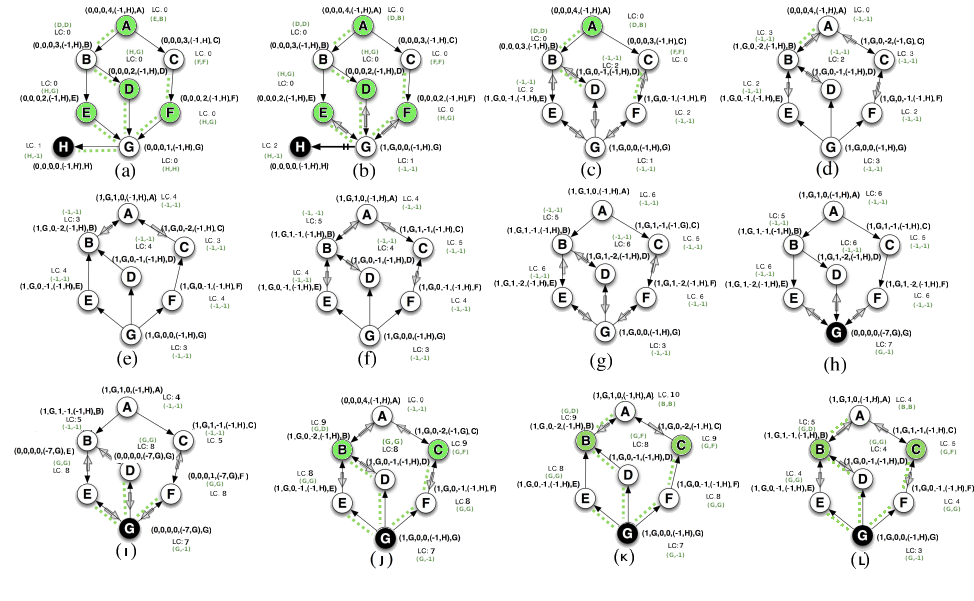
\includegraphics[width=1\linewidth]{test_1}
	\caption{}
	\label{fig:test1}
\end{figure}

\end{landscape}